\documentclass[conference]{IEEEtran}
\IEEEoverridecommandlockouts
% The preceding line is only needed to identify funding in the first footnote. If that is unneeded, please comment it out.
\usepackage{cite}
\usepackage{amsmath,amssymb,amsfonts}
\usepackage{algorithmic}
\usepackage{textcomp}
\usepackage{xcolor}
\usepackage{enumitem}
\usepackage{calc}
\usepackage{graphicx}
\usepackage[colorlinks=true,urlcolor=blue,linkcolor=green]{hyperref}
\graphicspath{{images/}}

\usepackage{lipsum}

\def\BibTeX{{\rm B\kern-.05em{\sc i\kern-.025em b}\kern-.08em
    T\kern-.1667em\lower.7ex\hbox{E}\kern-.125emX}}
    
\begin{document}

\title{Medify -- A medication reminder Android App}

\author{\IEEEauthorblockN{Ekrem Emre}
\IEEEauthorblockA{\textit{HTWG Konstanz -- University of Applied Sciences, Germany} \\
\textit{Matriculation number: 302110} \\
ek741emr@htwg-konstanz.de}
}

\maketitle

\begin{abstract}
\lipsum[1][1-4]
\end{abstract}

\section{Introduction}

\section{Goal of the project}

\section{Requirement analysis}

\subsection{Personas}
To simulate users for this application, two personas were created, which represents the user types
that might us this application.

\subsubsection{First persona} \hfill
\begin{figure}[htbp]
	\centerline{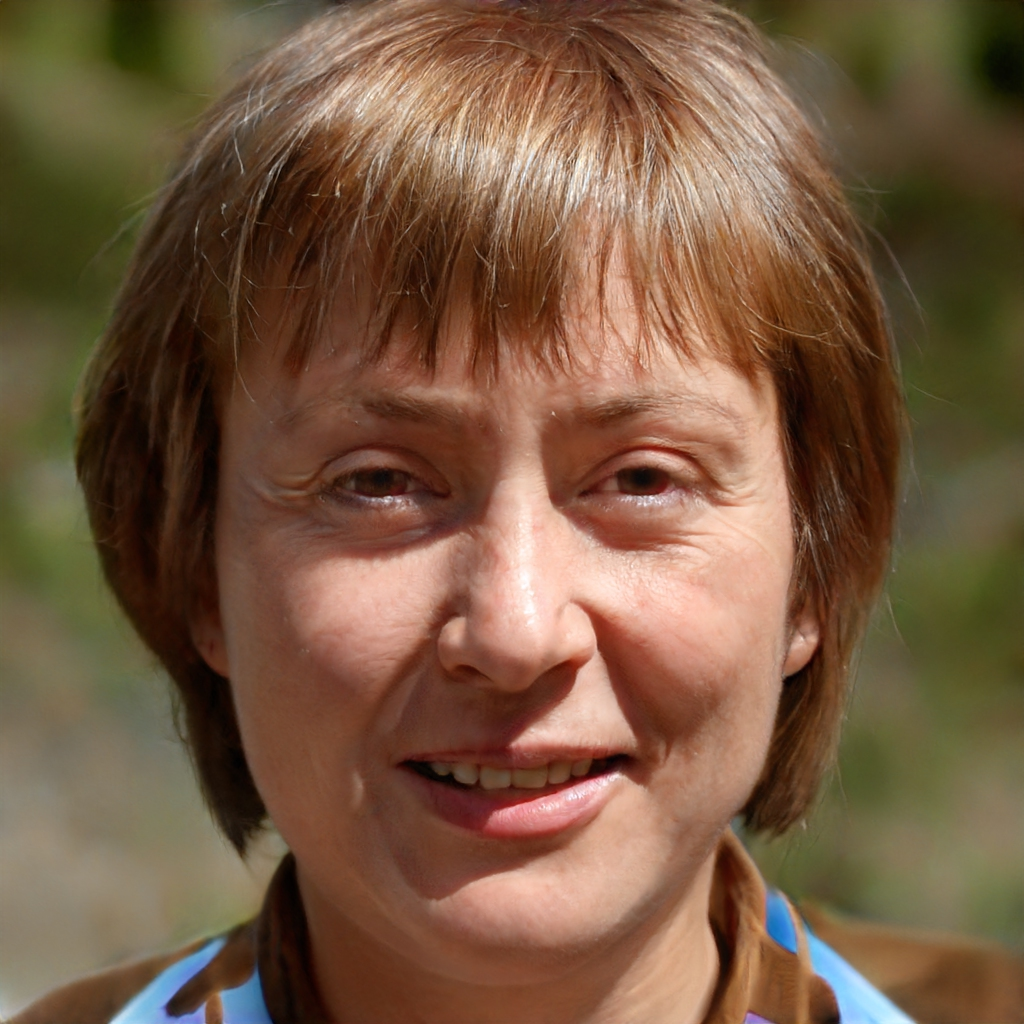
\includegraphics[width=.5\linewidth]{images/persona01.jpg}}
	\caption[Portrait of the persona Rosalyn Foster; Source taken from \cite{personaimg}]
	{\tabular[t]{@{}l@{}}Portrait of the persona Rosalyn Foster.\\ Source taken from \cite{personaimg}\endtabular}
	\label{fig:persona1}
\end{figure}

\begin{description}[labelwidth=\widthof{\bfseries Computer skills},leftmargin=.8cm,labelindent=.8cm]
	\item[Name] Rosalyn Foster
	\item[Age] 68
	\item[Marital status] Married
	\item[Occupation] Retiree
	\item[Computer skills] poor
\end{description}

\paragraph*{Key characteristics}
\begin{itemize}[leftmargin=1.25cm]
	\item Retiree, former tailor.
	\item Because of her advanced age, she got forgetful.
	\item Is regularly taking different medication, which she needs to be reminded of.
	\item Is concerned about her health, because she just became a grandparent and wants to spent as much time as possible with her grandchildren.
\end{itemize}

\paragraph*{Goals}
\begin{itemize}[leftmargin=1.25cm]
	\item Be healthy.
	\item Remember taking her medication regularly.
\end{itemize}

\paragraph*{User story}
As an older person, Rosalyn wants to be reminded to take her medicine, because she forgets them and wants to get healthy.

\subsubsection{Second persona} \hfill
\begin{figure}[htbp]
	\centerline{
\includegraphics[width=.5\linewidth]{images/persona02.jpg}}
	\caption[Portrait of the persona Christian Metz; Source taken from \cite{personaimg}]
	{\tabular[t]{@{}l@{}}Portrait of the persona Christian Metz.\\ Source taken from \cite{personaimg}\endtabular}
	\label{fig:persona2}
\end{figure}

\begin{description}[labelwidth=\widthof{\bfseries Computer skills},leftmargin=.8cm,labelindent=.8cm]
	\item[Name] Christian Metz
	\item[Age] 32
	\item[Marital status] Engaged
	\item[Occupation] Physiotherapist
	\item[Computer skills] strong
\end{description}

\paragraph*{Key characteristics}
\begin{itemize}[leftmargin=1.25cm]
	\item Working as a physiotherapist and doing a lot of sports, therefore is very healthy.
	\item He's a member in several sport clubs and a volunteer in the local animal shelter.
	\item His schedule is always pretty full and he's always on the go.
	\item He wants to increase his health by taking some vitamins, because he suspects he has some deficiencies.
\end{itemize}

\paragraph*{Goals}
\begin{itemize}[leftmargin=1.25cm]
	\item Be reminded, to take his vitamins.

\end{itemize}

\paragraph*{User story}
As a healthy person, Christian wants to be reminded to take his vitamins, because he's busy all day and not thinking of it and wants to stay healthy.

\subsubsection{Summary}
These personas show a user group, which are in need to take medication. However they struggle to 
remind themselves to take them in their daily lives.

\subsection{Storyboards}

\begin{figure*}[ht]
	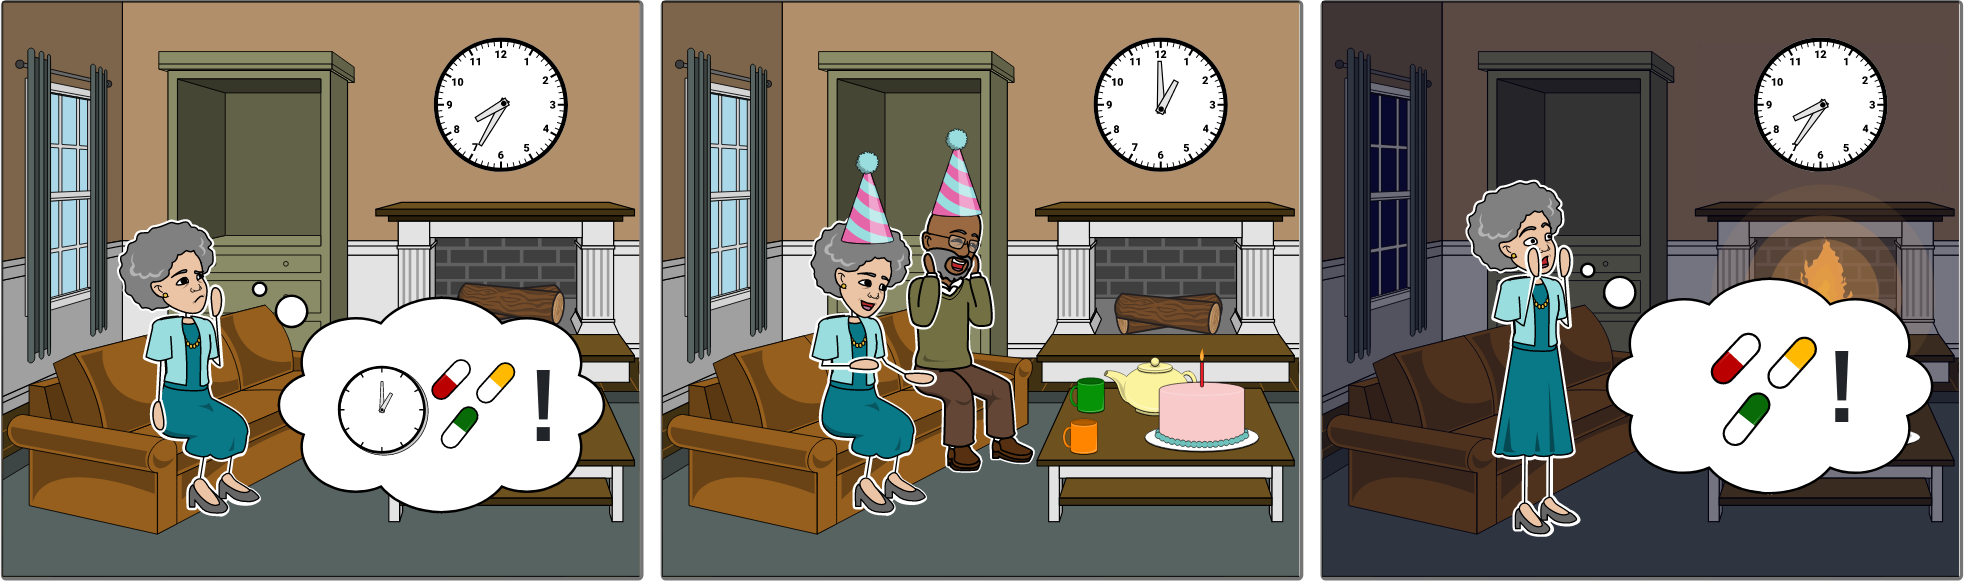
\includegraphics[width=\linewidth]{images/storyboard01.png}
	\caption
	{Storyboard showing an elderly person on her daily activities.
		In the first panel she reminds herself to take her medication at one o'clock.
		The second panel shows her enjoying her day with a friend, however she forgets to take her medicine.
		The last panel shows her in the evening and she realizes her blunder.
		Graphic created using \cite{storyboard}.}
	\label{fig:storyboard1}
\end{figure*}

\begin{figure*}[ht]
	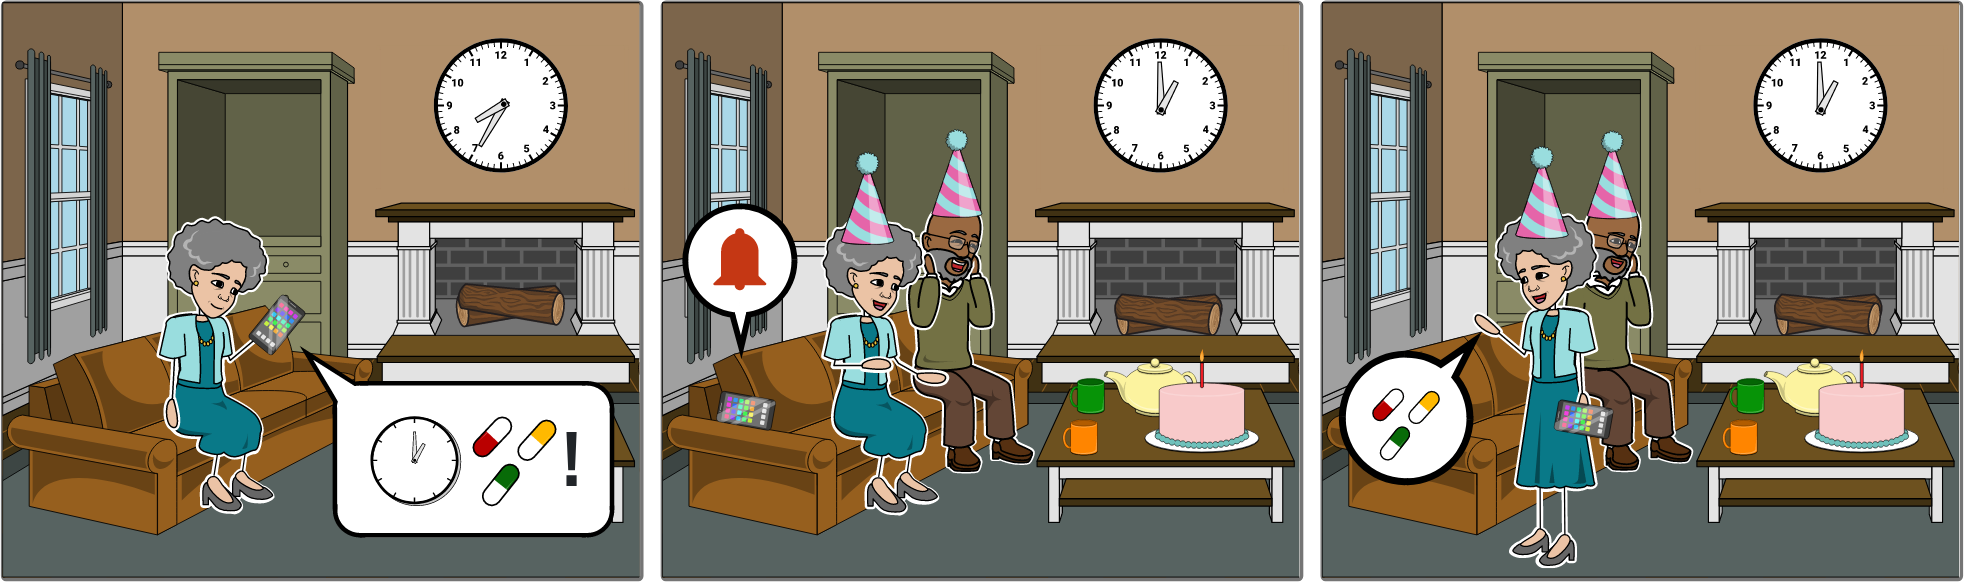
\includegraphics[width=\textwidth]{images/storyboard02.png}
	\caption
	{Storyboard showing an elderly person on her daily activities while using a medication reminder application.
		In the first panel she sets an alert on her smartphone, using the medication reminder app, at one o'clock.
		The second panel shows her and a friend enjoying their day. The medication reminder app alerts her at the set time, to take her medication.
		In the last panel she picks up her phone and takes her medication, just as advised by the application.
		Graphic created using \cite{storyboard}.}
	\label{fig:storyboard2}
\end{figure*}

To illustrate the practical use of a medication reminder application a storyboard was designed.
Fig. \ref{fig:storyboard1} shows an elderly person, which after some distractions in her daily
routine forgets to take her medicine.
Fig. \ref{fig:storyboard2} shows the same elderly person in a similar scenario. In order to manage
her medication, she uses her smartphone to get reminded when to take her medicine.



\section{Conceptual model of the solution}

\subsection{Entity relationship diagram}

\subsection{Activity diagram}

\subsection{Mockup}

\section{Design decisions}

\subsection{UML diagram}

\section{Results}

\section{Conclusion}


\begin{thebibliography}{00}	
	\bibitem{personaimg} P. Wang, ``This Person Does Not Exist,'' \textit{thispersondoesnotexist.com}, [Online] Available: \url{https://thispersondoesnotexist.com/} [Accessed Dec. 17, 2021].
	\bibitem{storyboard} Clever Prototypes, LLC, ``Storyboard That,'' \textit{storyboardthat.com}, [Online] Available: \url{https://www.storyboardthat.com/} [Accessed Dec. 17, 2021].
\end{thebibliography}

\end{document}

